
% ОБЯЗАТЕЛЬНО ИМЕННО ТАКОЙ documentclass!
% (Основной кегль = 14pt, поэтому необходим extsizes)
% Формат, разумеется, А4
% article потому что стандарт не подразумевает разделов
% Глава = section, Параграф = subsection
% (понятия "глава" и "параграф" из документа, описывающего диплом)
\documentclass[a4paper,article,14pt]{extarticle}

% Подключаем главный пакет со всем необходимым
\usepackage{spbudiploma_tempora}

% Пакеты по желанию (самые распространенные)
% Хитрые мат. символы
\usepackage{euscript}
% Таблицы
\usepackage{longtable}
\usepackage{makecell}
% Картинки (можно встявлять даже pdf)
\usepackage[pdftex]{graphicx}
\graphicspath{{figure_1/}{rgbcolor/}{figure_2/}}

\usepackage{amsthm,amssymb, amsmath}
% remove leading space of mod
\usepackage{textcomp}
\usepackage{enumitem}

\usepackage{float}


\newcommand{\Mod}[1]{\ \mathrm{mod}\ #1}

\begin{document}

% Титульник в файле titlepage.tex
% --------------------- Стандарт СПбГУ для ВКР --------------------------
% Автор: Тоскин Николай, itonik@me.com
% Если заметили ошибку, напишите на email
% Если хотите добавить изменение самостоятельно, GitHub: . PR-s welcome!
% Использованы материалы:
% habr.com/ru/post/144648/
% cpsconf.ru
% Текст:
% http://edu.spbu.ru/images/data/normativ_acts/local/20181030_10432_1.pdf
% Титульный лист:
% http://edu.spbu.ru/images/data/normativ_acts/local/20180703_6616_1.pdf
% -----------------------------------------------------------------------

% Титульный лист диплома СПбГУ
% Временное удаление foot на titlepage
\newgeometry{left=30mm, top=20mm, right=15mm, bottom=20mm, nohead, nofoot}
\begin{titlepage}
\begin{center}
% Первый символ съедается, первым знаком поставлен Ы
\textbf{Санкт--Петербургский}
\textbf{государственный университет}

\vspace{35mm}

\textbf{\textit{\large ПОТТЕР Гарри Джеймсович}} \\[8mm]
% Название
\textbf{\large Выпускная квалификационная работа}\\[3mm]
\textbf{\textit{\large Оптимизация заклятий в распределенной сети
мозгошмыг}}

\vspace{20mm}
% Булшит
Уровень образования: бакалавриат\\
Направление 01.03.02 «Прикладная математика и информатика»\\
Основная образовательная программа СВ.5005.2015
«Прикладная математика, фундаментальная информатика и программирование»\\
Профиль «Исследование и проектирование систем управления\\ и обработки сигналов»\\[30mm]


% Научный руководитель, рецензент
% Сходить в уч отдел и узнать, правильно ли
\begin{flushright}
{Научный руководитель:} \\
профессор, кафедра компьютерных технологий \\ и систем, д.ф. - м.н.  Веремей~Евгений Игоревич
\end{flushright}
\begin{flushright}
{Рецензент:} \\
профессор, кафедра компьютерных технологий \\и систем, д.ф. - м.н.  Веремей~Евгений Игоревич
\end{flushright}

\vfill 

{Санкт-Петербург}
\par{2019 г.}
\end{center}
\end{titlepage}
% Возвращаем настройки geometry обратно (то, что объявлено в преамбуле)
\restoregeometry
% Добавляем 1 к счетчику страниц ПОСЛЕ titlepage, чтобы исключить 
% влияние titlepage environment
\addtocounter{page}{1}

% Содержание
\tableofcontents
\pagebreak

\specialsection{Введение}
В настоящее время JavaScript является одним из самых популярных языков программирования. Он широко используется для создания приложений,
исполняемых и со стороны клиента в браузере, и со стороны сервера. Так же распространены нативные приложения для мобильных устройств, 
Progressive Web Apps - гибриды нативных приложений и сайтов. В первую очередь это связано с развитием интернета и увеличением объема
передаваемых по сети данных. Вместе с этим растет потребность в безопасности данных, которые представляют собой некоторую ценность.
Потребность передачи секретных данных возникает у ученых, военных, в судопроизводстве, бизнесе. 
Традиционные методы защиты информации предоставляет криптография. Чаще всего информация защищается с помощью секретного алгоритма или ключа.
Но у такого подхода есть проблемы: если злоумышленник перехватит ключ или скомпрометирует одну из сторон, то он легко получит доступ к секрету.
Также, при необходимости разделить секретную информацию между какой-то группой людей приходится устанавливать соединения между каждой парой из группы,
что негативно сказывается на безопасности секрета.

В 1979 году A. Shamir представил \cite{shamir} алгоритм 
разделения секрета, который позволяет разбить секрет на $n$ долей таким образом, что знание $K$ и более долей позволяет восстановить 
секрет, а знание $K-1$ и менее долей делает восстановление секрета невозможным. В последние десятилетия было предложено множество 
алгоритмов разделения секрета для электронных изображений. В данной работе будет рассмотрен алгоритм обратимого 
разделения секрета для изображения в оттенках серого и адаптирован для использования с цветными секретными изображениями,
реализована библиотека для использования в веб-приложениях и пример минимального проекта, использующего эту 
библиотеку.

Исходя из вышесказанного, актуальность работы заключается в необходимости разработки программных средств с открытым исходным кодом
для обеспечения безопасности веб-приложений с возможностью разделения секретного изображения на несколько частей.
% Открытый исходный код
% позволяет пользователям убедиться в отсутствии вредоносных скриптов, уязвимостей, дает возможность искать ошибки и дополнять код сообществу разработчиков.
%, в связи с отсутствием 

\newpage
\specialsection{Цель и постановка задачи}

Целью данной работы является написание библиотеки для языка JavaScript, для разделения секретного цветного электронного изображения,
с долями, не подобными шуму. Для достижения этой цели были поставлены следующие задачи:
\begin{enumerate}
    \item Исследование предметной области;
    \item Выбор алгоритма;
    \item Модификация алгоритма для работы с цветным секретным изображением;
    \item Написание библиотеки;
    \item Написание минимального веб-приложения, позволяющего продемонстрировать работу программы;
    \item Тестирование библиотеки.
\end{enumerate}

\newpage
\specialsection{Обзор литературы}
Основной работой является схема разделения секрета Шамира \cite{shamir}, более подробно рассмотренная в следующей главе.

Статья \flqq An investigation on image secret sharing\frqq \cite{review} структурирует разновидности модификаций схемы Шамира и содержит многие выдержки из современных работ.

Основным алгоритмом в этой работе является Reversible Image Secret Sharing \cite{RISS} из одноименной статьи. Этот агоритм является модификацией
алгоритма, прeдставленного в статье Chinese remainder theorem-based secret image sharing for (k,n) threshold \cite{CRTSIS}, для использования
с изображениями прикрытия.

При работе использовался ресурс Scopus \cite{scopus} для поиска научных статей. 
    Для имплементации библиотеки и веб-приложения использовались open-source библиотеки и документации
\cite{react} \cite{image-js} \cite{Big.js} к ним.

\newpage
\section{Исследование предметной области}
Одним из первых алгоритмов разделения секрета является (k, n) пороговая схема Шамира\cite{shamir}. В ее основе лежит интерполяция 
полиномов. Пусть $D$ -- некоторая секретная информация, представленная в форме числа. Выберем простое число $p: p > D, p > N$.
Чтобы разделить секрет на $n$ частей возьмем случайный полином степени $k-1$ 
\begin{equation}
    q(x) = a_0 + a_1 x +...+ a_{k-1} x^{k-1},
    a_0=D, a_i<p
\end{equation}
и вычислим
\begin{equation}
    D_1=q(1)\Mod{p}, ..., D_i=q(i)\Mod{p}, ..., D_n=q(n)\Mod{p}
\end{equation}
Число $p$ будет публичным для всех участников, числа $D_i$ назовем долями. Участника схемы, который хочет разделить секрет и 
формирует доли назовем дилером.

Имея $k$ и более долей, можно восстановить секрет $D$ при помощи полиномиальной интерполяции.
%добавить инфу про восстановление 

Допустим, злоумышленнику удалось получить доступ к $k-1$ долям, тогда для каждого $D': 0<D'<p$ он может восстановить единственный полином степени $k-1$, такой, что $q_0=D'$ и 
$q_i=D_i$. Так как $a_i$ случайны, эти $p$ полиномов с одинаковой вероятностью являются искомыми, злоумышленник не получает никакой
информации о секрете. 

Схема Шамира позволяет разделить секрет, представленный в форме числа и используется в основном для защиты ключей. Изображение так же 
можно представить в форме числа, но при обычном размере изображения (для примера 256х256) и значениях пикселя (0-255)х3 для RGB изображений
будет тратиться огромное количество памяти и возрастет время генерации долей и восстановления секрета. Поэтому на основе схемы Шамира были разработаны алгоритмы разделения секрета для изображений. 
Их можно разделить на три категории - схемы визуальной криптографии(VCS), полиномиальные схемы и схемы, основанные на Китайской теореме об остатках. 

В 1994 году Moni Naor и Adi Shamir \cite{shamir_VCS} представили первую VCS, на ее основе были разработаны другие модификации.
В VCS схемах доли обычно печатаются на прозрачных носителях и секрет восстанавливается путем наложения частей друг на друга. 
Основным преимуществом таких схем является отсутствие необходимости вычислений при восстановлении секрета.
Примечательной для применения в веб-разработке является VCS схема WEB-VC \cite{WEB-VC}. Алгоритм восстановления секрета в ней основан 
на возможности установить прозрачность элемента в таблице каскадных стилей (CSS). Основными недостатками таких схем являются 
наличие помех в восстановленном секретном изображении и возможность использования только с бинарными изображениями.

Полиномиальные схемы используются чаще из-за лучшего качества восстановленного секрета и в общем случае 
не требуют увеличения количества пикселей. Но у них есть и недостатки -- относительно высокая вычислительная сложность 
восстановления секрета $O(k \times log^2(k))$ для каждого пикселя и небольшие потери в качестве восстановленного секретного изображения.
% Дополнить про 1 достойную схему

Схемы, основанные на Китайской теореме об остатках имеют более низкую сложность операции восстановления $O(k)$ и позволяют 
восстановить секрет без потерь. Недостатком таких схем является ограниченное количество участников\cite{CRTSIS}. Таким образом, 
эти схемы отлично подходят для устройств с низкой вычислительной мощностью и для использования в веб-приложениях.

Во многих схемах дилер отправляет участникам шумо-подобные доли. Введём понятие изображений для прикрытия -- это произвольные 
изображения, использующиеся для генерации долей. Сгенерированные доли являются изображениями, похожими на изображения прикрытия. 
Использование изображений прикрытия вместо шумо-подобных долей снижает риск привлечения внимания к долям злоумышленников, улучшает возможности 
по их менеджменту. 

В данной работе будет рассматриваться алгоритм Reversible Image Secret Sharing \cite{RISS}. Он основан на китайской 
теореме об остатках. В качестве секретной картинки выступает изображение в оттенках серого $(0-255)$, картинками для прикрытия являются
бинарные изображения.


\newpage
\section{Описание алгоритма}
Начнем описание работы алгоритма с формулировки Китайской теоремы об остатках.

Если $ a_1,...,a_n \in N $ попарно взаимно просты, то для 
$$\forall r_1,...,r_n \in N : 0\leq r_i<a_i, \forall i\in \overline{1,n}$$
найдется $N: N \Mod a_i = p_i, \forall i\in \overline{1,n}$ 

Эта теорема позволяет за линейное время решать систему линейных модулярных уравнений следующего типа:
\begin{gather}
    \begin{cases}
    y \equiv a_1 \Mod m_1 \\
    y \equiv a_2 \Mod m_2 \\
    ... \\
    y \equiv a_k \Mod m_k
    \end{cases}
\end{gather}
\hypertarget{CRTSolve}{Алгоритм решения:}
\begin{enumerate}
    \item Вычисляем $M=\prod\limits_{i = 1}^k m_i$;
    \item $\forall i\in \overline{1,k}$ вычисляем $M_i={{M} \over {m_i}}$;
    \item С помощью расширенного алгоритма Евклида $\forall i\in \overline{1,k}$ находим ${M_i}^{-1}$ обратное по модулю для $M_i$;
    \item Получаем $y \equiv \sum\limits_{i=1}^k a_i M_i {M_i}^{-1} \Mod M$.
\end{enumerate}

Предложенный алгоритм состоит из двух частей: формирование долей и восстановление секрета. Опишем их более подробно.

\subsection{Формирование долей}
Описание входных данных:

\begin{itemize}
    \setlength{\itemindent}{3em}
    \item Секретное изображение $S$ размера $W_S \times H_S$ пикселей в оттенках серого (значения пикселей 0-255);
    \item $n$ - количество долей;
    \item $k$ - минимальное количество долей для восстановления секрета;
    \item $n$ изображений $C_i$ размера $W_S \times H_S$ - бинарные (значения пикселей 0-1) изображения прикрытия для каждого из участников.
\end{itemize}

Описание выходных данных:

\begin{itemize}
    \setlength{\itemindent}{3em}
    \item $n$ изображений $SC_i$ размера $W_S \times H_S$ - сгенерированные доли;
    \item $m_i$ - приватное число для каждой доли;
    \item $p, T$ - публичные для всех участников числа для восстановления секрета.
\end{itemize}

\hypertarget{generation_alg}{Алгоритм}:
\begin{enumerate}
    \setlength{\itemindent}{3em}
    \item Выберем число $p$ и $n$ взаимно простых чисел $m_i$ таких, что 
    $$128 \leq p < m_i \leq 256, \text{НОД}(m_i, p)=1, \forall i \in \overline{1,n}$$ 
    \item Вычислим $M=\prod\limits_{i = 1}^k m_i$, $N=\prod\limits_{i = 1}^{k-1} m_{n-i+1}$
    \item Если $M<pN$ перейдем к шагу 1
    \item Вычислим $T=\left[ {{\left\lfloor{{M}\over{p}}-1\right\rfloor}\over{2}} \right]$
    \item Для каждого секретного пикселя $x$ с координатами $[w, h]$ повторяем шаги 6-7
    \item \hypertarget{step6_1}{Если} $0 \leq x < p$, выберем случайное $ A \in \left[T+1, {\left\lfloor{{M} \over {p}} - 1\right\rfloor}\right]$ и вычислим
    $y = x + Ap$. 
    
    Если $x \geq p$ выберем случайное $ A \in [0, T)$ и вычислим $y = x - p + Ap$
    \item Если выполняется одно из следующих условий, то вычисляем $a_i = y \Mod p$, устанавливаем $SC_i=a_i$ и
    переходим к следующему пикселю, иначе возвращаемся на шаг 6.
    \begin{gather}
        \begin{cases}
        SC_i[w,h] \geq TH_{i1}, \text{ если } C_i[w,h] = 1 \\
        SC_i[w,h] \leq TH_{i0}, \text{ если } C_i[w,h] = 0
        \end{cases}
    \end{gather}
    \begin{equation}
        \text{при } TH_{i0} = {{m_i} \over 2} - TH,\text{ } TH_{i1} = {{m_i} \over 2} + TH
    \end{equation}
\end{enumerate}

\subsection{Восстановление секрета}

Описание входных данных:
\begin{itemize}
    \setlength{\itemindent}{3em}
    \item $n$ долей $SC_i$ ($n \geq k$) и соответствующие им $m_i$
    \item Публичные числа $T, p$
\end{itemize}

Описаные выходных данных:
\begin{itemize}
    \setlength{\itemindent}{3em}
    \item Восстановленный секрет $S'$
    \item Восстановленные изображения прикрытия $C_{i}'$ размера $[W_S, H_S]$
\end{itemize}

\hypertarget{recover_alg}{Алгоритм}
\begin{enumerate}
    \setlength{\itemindent}{3em}
    \item Восстановливаем изображения прикрытия с помощью бинаризации. Для каждого пикселя $C_{i}'[w, h]$ устанавливаем значение 
    $$\text{Если } SC_{i}[w, h]>{{m_i}\over{2}} \text{, то } 1 \text{, иначе } 0$$
    \item Для каждой позиции пикселя $[w, h]$, $a_i = SC_i[w, h]$, с помощью \hyperlink{CRTSolve}{описанного выше алгоритма} решаем систему 
    линейных уравнений по модулю:
    \begin{gather}
        \begin{cases}
        y \equiv a_1 \Mod m_1 \\
        y \equiv a_2 \Mod m_2 \\
        ... \\
        y \equiv a_n \Mod m_n
        \end{cases}
    \end{gather}
    \item Вычисляем $T^{*}=\left\lfloor{{y} \over {p}}\right\rfloor$. Если $T^{*}\leq T$, то $x = y \Mod p$, иначе $x = (y \Mod p) + p$.
    
    $S'[w, h] = x$
\end{enumerate}

\subsection{Комментарии к алгоритму}
\begin{enumerate}
    \item Число $p$ в \hyperlink{generation_alg}{алгоритме 1} выбирается наименьшим из возможных, а числа $m_i$ выбираются наибольшими для достижения 
    большего диапазона распределения значения пикселя в долях.

    \item \hypertarget{comments}{Параметр $TH$} имеет весомую роль в качестве сгенерированных долей, времени генерации и безопасности. Этот параметр устанавливается 
    дилером и влияет на $N_A$ -- число возможных значений А в \hyperlink{step6_1}{шаге 6 алгоритма 1}.
    В общем случае, $N_A = T$. Для того, чтобы удовлетворять условию на шаге 7 алгоритма, значение $N_A$ уменьшается до 
    $N_A = T \times \prod\limits_{i = 1}^n \left({1\over 2} \times {TH_{i0}\over m_i} + {1\over 2} \times {{m_i - TH_{i0}}\over m_i}\right)$.
    
    При увеличении $TH$ уменьшается $N_A$, увеличивается качество сгенерированных долей и время на генерацию.
    При увеличении $N_A$ улучшается безопасность, так как количество значений для перебора равняется $T^{N_A}$. 
    Требуется, чтобы $N_A \geq 2$, так как при $N_A = 1$ в шаге 6 алгоритма будет 
    повторно использоваться одно и то же значение $A$, что приводит к проблемам с безопасностью. Экстремальной точкой для качества долей 
    является $TH = 112$. Экспериментальные данные можно увидеть на Рисунке~(ссылка). 

    \item Качество картинки по сравнению с изначальной будем измерять с помощью пикового отношения сигнала к шуму -- $PSNR$. Эту метрику чаще всего 
    определяют с помощью среднеквадратичной ошибки $MSE$ \cite{metrics}. Пусть $I$ -- исходное изображение размера $m \times n$, $K$ -- зашумленная версия $I$. Тогда 
    \begin{equation}
        MSE = {1\over mn} \sum_{i=0}^{m-1} \sum_{j=0}^{n-1}{|I[i, j] - K[i, j]|}^2
    \end{equation}
    \begin{equation}
        PSNR = 10 \log_{10}\left({{MAX_i^2} \over {MSE}} \right)
        \label{eq:RSNR}
    \end{equation}

    \item Мощностью встраивания $EC$ (embedding capacity) \cite{metrics} называется отношение количества бит информации, встраиваемых в изображение, к размеру изображения 
    и определяется формулой:
    $$EC = {N\over{L\times H \times W}}$$
    $N$ -- число бит секрета, $L$ -- количество бит в пикселе, $H \times W$ -- размер изображения.
    
    Для данного алгоритма $EC$ примет следующий вид:
    \begin{equation}
        EC = {{(L_S \times W_S \times H_S) + (n_C \times L_C \times W_C \times H_C)} \over
            {n_{SC} \times L_{SC} \times W_{SC} \times H_{SC}}}
        \label{eq:EC}  
    \end{equation}
    где $S$ -- секретное изображение, $C$ -- изображения прикрытия, $SC$ -- доли, $L_x$ - количество бит в пикселе,
    $W_x, \text{ } H_x$ -- ширина и высота, $n_x$ -- количество изображений.
    
    Таким образом, $L_S=L_{SC}=8$, $L_C=1$, $W_S=W_C=W_SC=W$, $H_S=H_C=H_SC=H$, $n_C=n_{SC}=n$
    \begin{equation}
        EC = {{(8 \times W \times H) + (n \times W \times H)} \over
            {8 \times n \times W \times H}} =
            {{8+n}\over{8n}}
    \end{equation}
    \item Результаты работы алгоритма для изображений, размером $512\times 512$ $n=5$, $k=4$, $TH=16$ показаны на Рисунке~\ref{fig:experimental_grey_images}.
    Значения $PSNR$ -- $SC_1$: $37.36$, $SC_2$: $37.15$, $SC_3$: $36.93$, $SC_4$: $37.25$, $SC_5$: $36.98$  
\end{enumerate}
\begin{figure}[H]
    \begin{minipage}[h]{0.3\linewidth}
        \center{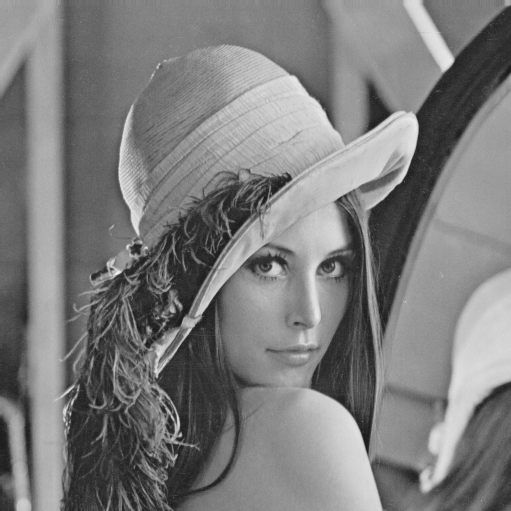
\includegraphics[width=1\linewidth]{lena.png} \\ $S$ }
    \end{minipage}
    \begin{minipage}[h]{0.3\linewidth}
        \center{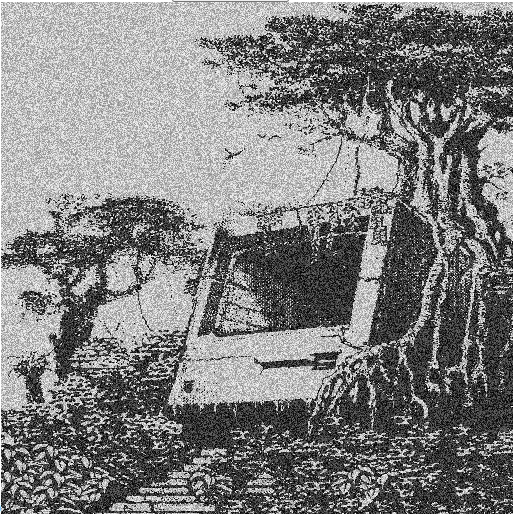
\includegraphics[width=1\linewidth]{share1.png} \\ $SC_1$ }
    \end{minipage}
    \begin{minipage}[h]{0.3\linewidth}
        \center{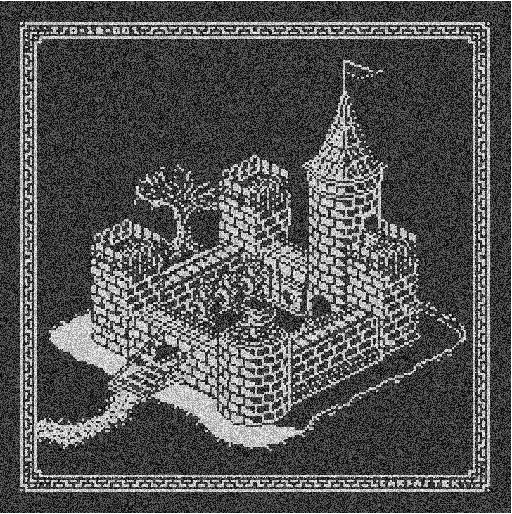
\includegraphics[width=1\linewidth]{share2.png} \\ $SC_2$}
    \end{minipage}
    \begin{minipage}[h]{0.3\linewidth}
        \center{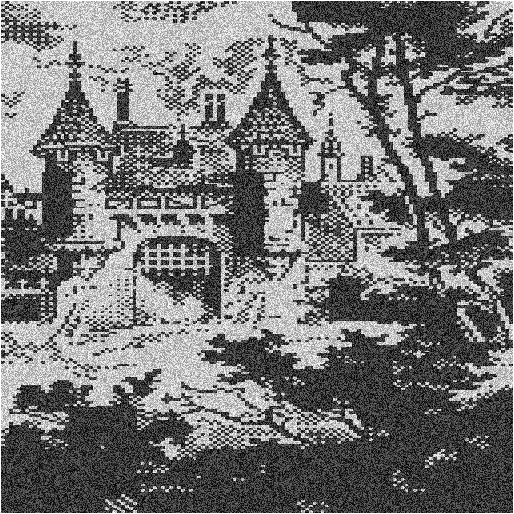
\includegraphics[width=1\linewidth]{share3.png} \\ $SC_3$}
    \end{minipage}
    \begin{minipage}[h]{0.3\linewidth}
        \center{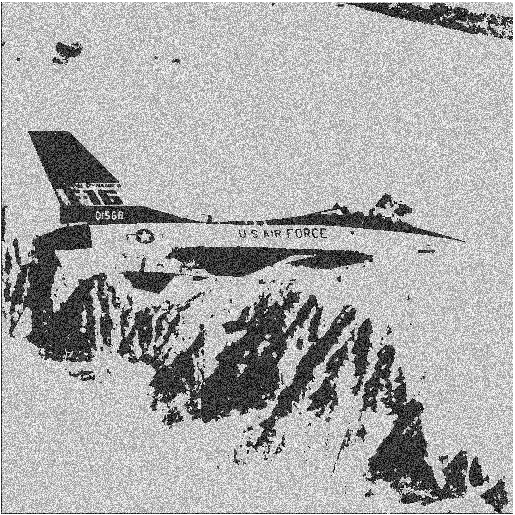
\includegraphics[width=1\linewidth]{share4.png} \\ $SC_4$}
    \end{minipage}
    \begin{minipage}[h]{0.3\linewidth}
        \center{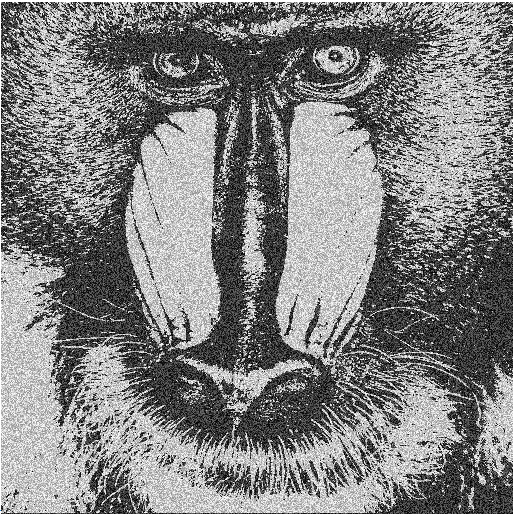
\includegraphics[width=1\linewidth]{share5.png} \\ $SC_5$}
    \end{minipage}
    \begin{minipage}[h]{0.3\linewidth}
        \center{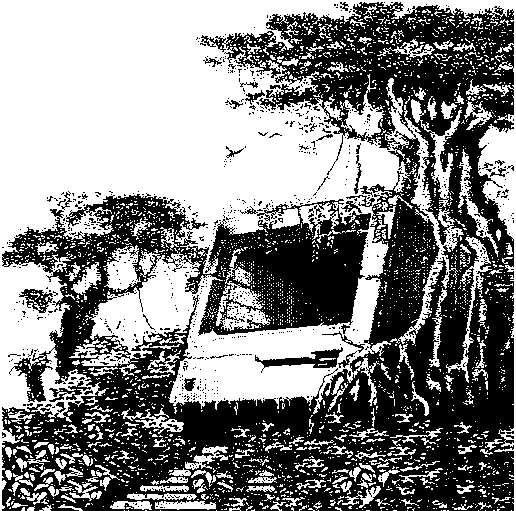
\includegraphics[width=1\linewidth]{binary1.png} \\ $C_{1}'=C_{1}$ \\ $PSNR=\infty$}
    \end{minipage}
    \begin{minipage}[h]{0.3\linewidth}
        \center{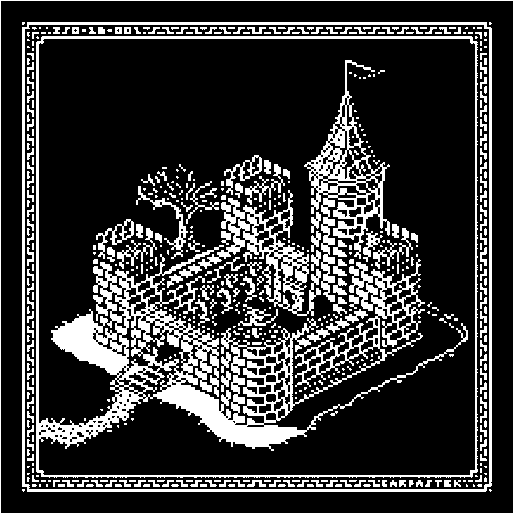
\includegraphics[width=1\linewidth]{binary2.png} \\ $C_{2}'=C_{2}$ \\ $PSNR=\infty$}
    \end{minipage}
    \begin{minipage}[h]{0.3\linewidth}
        \center{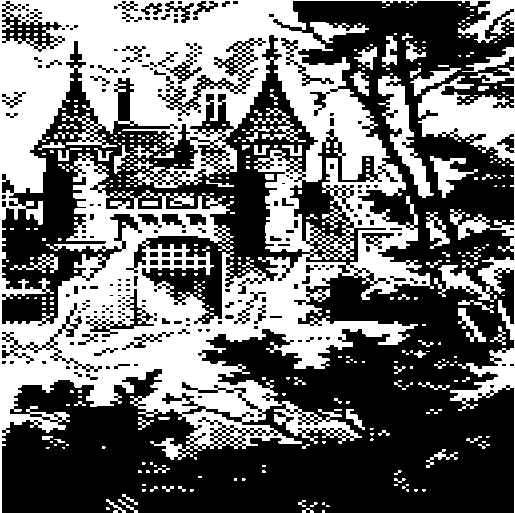
\includegraphics[width=1\linewidth]{binary3.png} \\ $C_{3}'=C_{3}$ \\ $PSNR=\infty$}
    \end{minipage}
    \begin{minipage}[h]{0.3\linewidth}
        \center{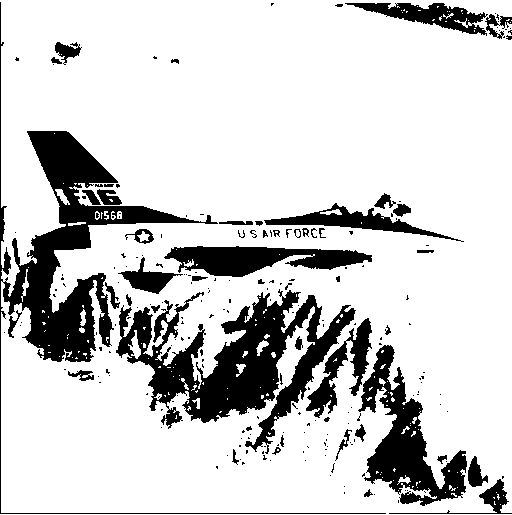
\includegraphics[width=1\linewidth]{binary4.png} \\ $C_{4}'=C_{4}$ \\ $PSNR=\infty$}
    \end{minipage}
    \hfill
    \begin{minipage}[h]{0.3\linewidth}
        \center{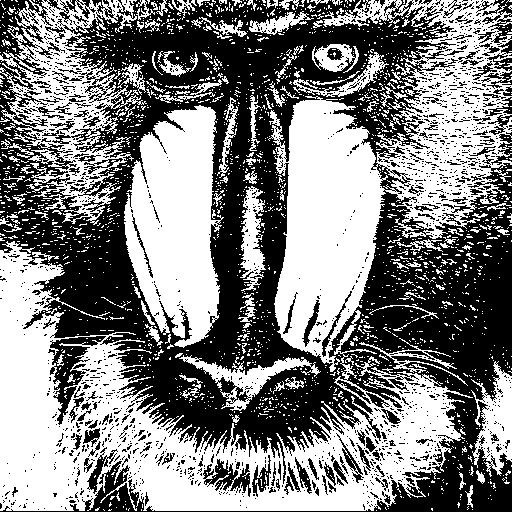
\includegraphics[width=1\linewidth]{binary5.png} \\ $C_{5}'=C_{5}$ \\ $PSNR=\infty$}
    \end{minipage}
    \hfill
    \begin{minipage}[h]{0.3\linewidth}
        \center{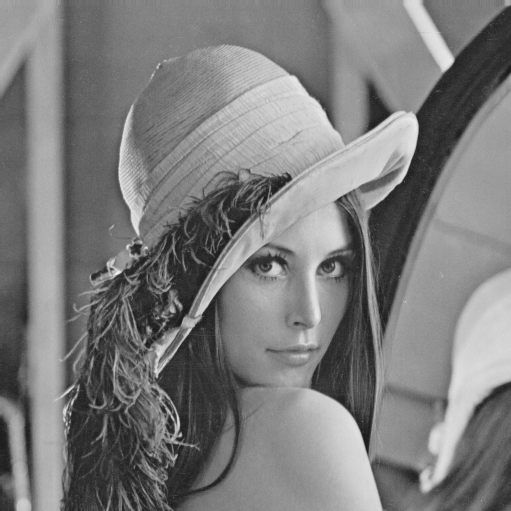
\includegraphics[width=1\linewidth]{lena.png} \\ $S_{1234}'=S_{2345}'=S$ \\ $PSNR=\infty$ }
    \end{minipage}
    \caption{Экспериментальные изображения}
    %задает метку рисунка чтобы после ссылаться
    \label{fig:experimental_grey_images}
\end{figure}

% \newpage
\section{Модификация алгоритма}

Описанный выше алгоритм отлично подходит для цели работы, за исключением цвета секретной картинки. Поэтому
было принято решение расширить исходный алгоритм для использования с цветными секретными картинками. 
Это было достигнуто с помощью увеличения количества пикселей в картинках прикрытия и кодирования каждого канала цвета 
в определенном пикселе доли. Схема расположения каналов в доле представлена на Рисунке~\ref{fig:channels}. 

Каждый пиксель секретного изображения кодируется в 4 пикселях картинки прикрытия.
Размер исходной цветной картинки -- $2\times 1$, размер доли и размер картинки прикрытия -- $8 \times 1$.
Белый сегмент при использовании с картинками формата rgba отвечает за кодирование канала прозрачности alpha,
для rgb не принимает участия в разделении секрета и в зависимости от значения пикселя картинки прикрытия $C_{ij} = 0 | 1$ принимает значения $0 | 255$.

\begin{figure}[H]
    \center{
\includegraphics[width=1\linewidth]{rgba.png}}
    \caption{Схема расположения каналов}
    \label{fig:channels}
\end{figure}

Изображения в коде веб-приложения и при передаче между клиентом и сервером хранятся в форме массива бит. 
Для того, чтобы избежать существенного увеличения размера изображения на диске, доли можно сохранять в формате $PGM$ -- portable gray map. В нем для 
кодирования каждого пикселя используется 8 бит. Таким образом, изображение доли будет занимать на диске и в памяти такое же пространство, как и секретное rgba изображение.

Рассмотрим метрику EC (\ref{eq:EC}) для дополненного алгоритма. Для RGBA изображения: 
$$EC = {{(32 \times {W \over 2} \times {H \over 2}) + (n \times W \times H)} \over
{n \times 8 \times W \times H}} = {8+n \over 8n}$$
Для RGB изображения:
$EC = {6+n \over 8n}$

Результаты работы алгоритма с цветным секретным изображением размера $256\times256$, $n=4$, $k=3$ представлены на Рисунке~\ref{fig:experimental_mod}.

\begin{figure}[ph!]
    \begin{minipage}[h]{0.3\linewidth}
        \center{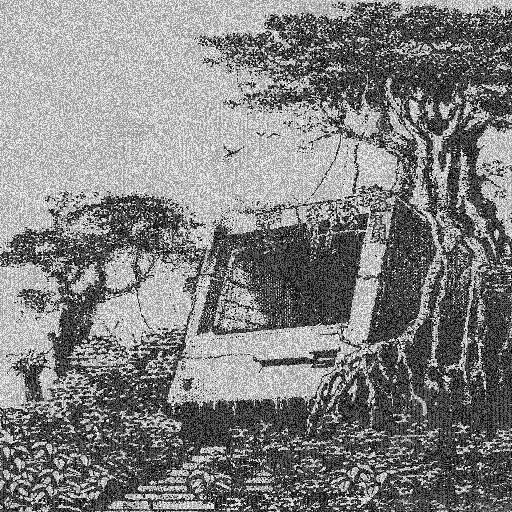
\includegraphics[width=1\linewidth]{COLshare1.png} \\ $SC_1$ \\ $PSNR=\infty$}
    \end{minipage}
    \hfill
    \begin{minipage}[h]{0.3\linewidth}
        \center{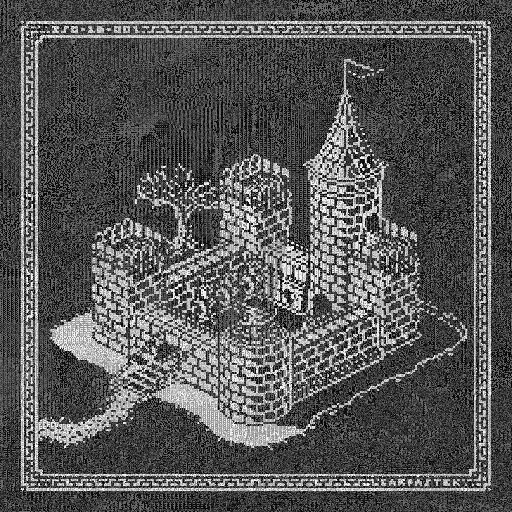
\includegraphics[width=1\linewidth]{COLshare2.png} \\ $SC_2$ \\ $PSNR=\infty$}
    \end{minipage}
    \hfill
    \begin{minipage}[h]{0.3\linewidth}
        \center{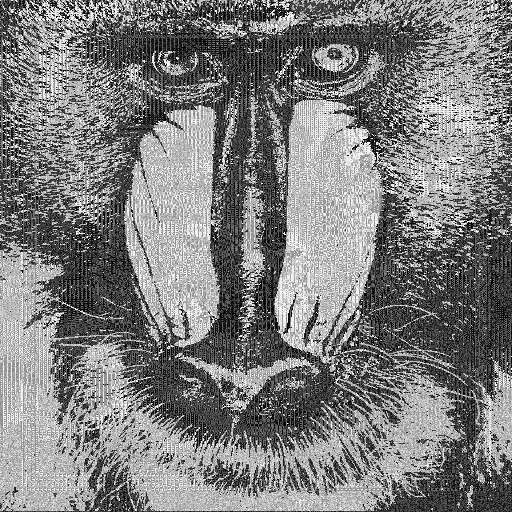
\includegraphics[width=1\linewidth]{COLshare3.png} \\ $SC_3$ \\ $PSNR=\infty$}
    \end{minipage}
    \vfill
    \begin{minipage}[h]{0.3\linewidth}
        \center{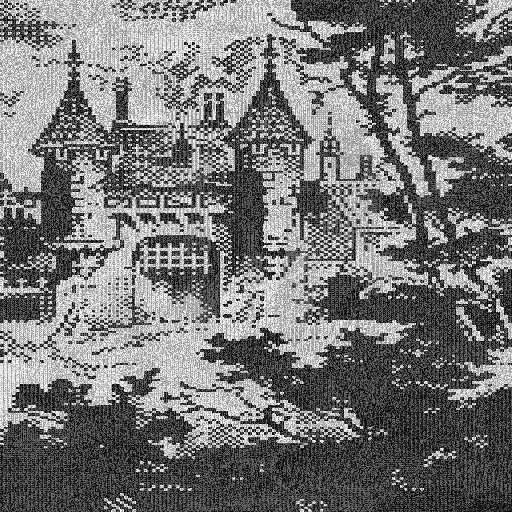
\includegraphics[width=1\linewidth]{COLshare4.png} \\ $SC_4$ \\ $PSNR=\infty$}
    \end{minipage}
    \hfill
    \begin{minipage}[h]{0.3\linewidth}
        \center{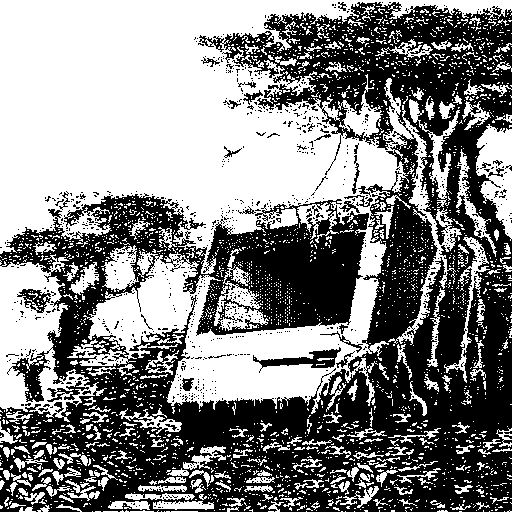
\includegraphics[width=1\linewidth]{cover1.png} \\ $C_{1}'=C_{1}$ \\ $PSNR=\infty$}
    \end{minipage}
    \hfill
    \begin{minipage}[h]{0.3\linewidth}
        \center{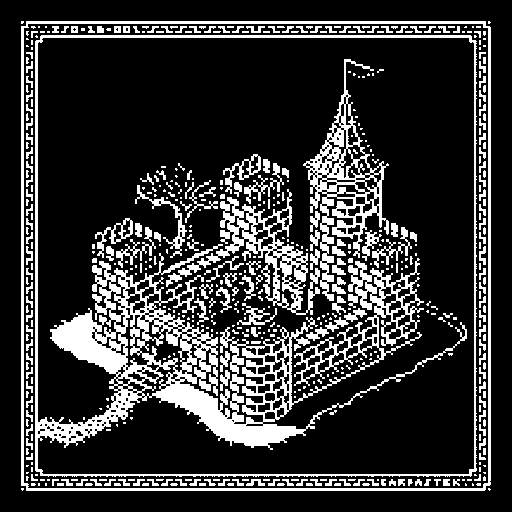
\includegraphics[width=1\linewidth]{cover2.png} \\ $C_{2}'=C_{2}$ \\ $PSNR=\infty$}
    \end{minipage}
    \vfill
    \begin{minipage}[h]{0.3\linewidth}
        \center{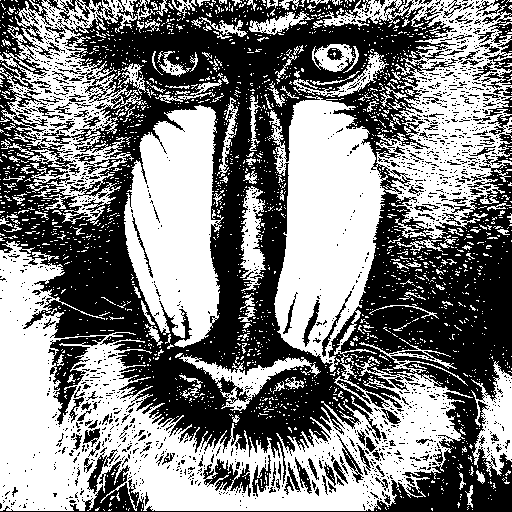
\includegraphics[width=1\linewidth]{cover3.png} \\ $C_{3}'=C_{3}$ \\ $PSNR=\infty$}
    \end{minipage}
    \hfill
    \begin{minipage}[h]{0.3\linewidth}
        \center{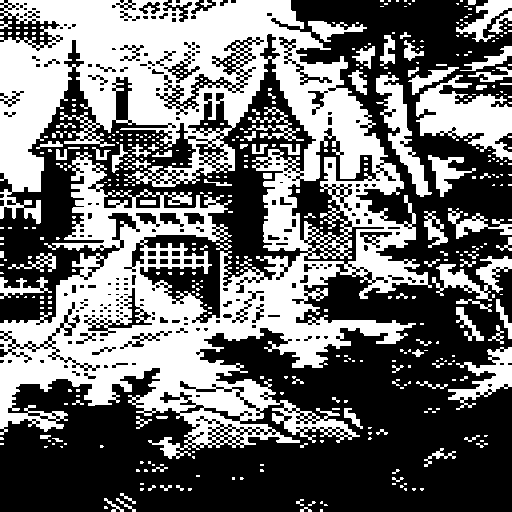
\includegraphics[width=1\linewidth]{cover4.png} \\ $C_{4}'=C_{4}$ \\ $PSNR=\infty$}
    \end{minipage}
    \hfill
    \begin{minipage}[h]{0.3\linewidth}
        \center{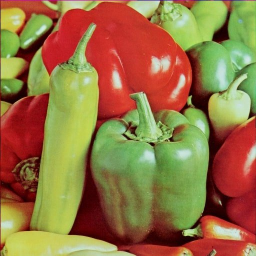
\includegraphics[width=1\linewidth]{pepper256.png} \\ $S_{1234}'=S_{2345}'=S$ \\ $PSNR=\infty$ }
    \end{minipage}
    \caption{Результаты работы для цветного изображения}
    %задает метку рисунка чтобы после ссылаться
    \label{fig:experimental_mod}
\end{figure}

\newpage
\section{Имплементация библиотеки}

В ходе работы была написана библиотека на языке JavaScript, которая реализует работу \hyperlink{generation_alg}{алгоритма 1 } и адаптирует его для
работы с цветными изображениями. 
На данный момент в открытом доступе есть две библиотеки, реализующие схему Шамира для числа: \flqq shamir-secret-sharing\frqq и \flqq secrets.js\frqq,
но, как было отмечено выше, они подходят только для кодирования секрета в форме числа. Для изображений
имплементации на языке JavaScript каких-либо алгоритмов разделения секрета отсутствуют.
Основным преимуществом данной библиотеки является возможность ее использования как со стороны клиента, так и со стороны сервера.

Для улучшения безопасности, все данные следуюет передавать по HTTPS (HyperText Transfer Protocol Secure) - протоколу зашифрованной передачи данных.
Если важна скорость работы, например для передачи большого количества изображений, то генерацию долей лучше производить на сервере. 
Если важнее стоит безопасность, то генерацию можно провести в клиентском приложении и отправлять доли по более защищенным каналам.
Исключение сервера из процесса генерации снижает возможность атаки MITM(man in the middle). Таким образом, у злоумышленника есть
только 3 варианта получения доступа к секрету - получение доступа к машине дилера, получение доступа к $K$ частям секрета и полный перевбор значений.
Последние 2 варианта являются тяжело реализуемыми на практике, поэтому основной уязвимостью системы является дилер.

Библиотека написана в функциональном стиле, все функции не обладают побочными эффектами.
Установка осуществляется с помощью пакетного менеджера npm.

В языке JavaScript изначально не предусмотрена возможность работы с длинной арифметикой, поэтому в проекте используется библиотека
с открытым исходным кодом "Big.js". Она предоставляет интерфейс Big, со структурой для хранения информации о числе и методами, 
реализующими базовый набор арифметических операций.

Основными функциями являются encrypt и recover. Они представляют собой работу \hyperlink{generation_alg}{алгоритмов 1} и \hyperlink{recover_alg}{2} соответственно. 
Рассмотрим их подробнее.

В функции encrypt входными параметрами являются:
\begin{enumerate}[leftmargin=2cm]
    % \setlength{\itemindent}{3em}
    \item sharesNum - число участников схемы;
    \item threshold - пороговое число участников для восстановления секрета
    \item secretPixels - одномерный массив со значениями пикселей секретного изображения;
    \item covers - массив из sharesNum картинок прикрытия, представленных в форме одномерного массива;
    \item TH - параметр, подробнее в \hyperlink{comments}{главе 2.3}.
\end{enumerate}
Изображения представляются в виде одномерного массива для удобства работы с индексами в случае работы с RGB и RGBA форматами.

Выходные данные:

\begin{enumerate}[leftmargin=2cm]
    \item modifiedCovers - доли, отправляемые участникам;
    \item m - массив приватных чисел, соответствующих каждому из учатников;
    \item T, p - публичные для всех участников числа.
\end{enumerate}

В теле encrypt используются следующие функции: 
\begin{itemize}
    \setlength{\itemindent}{2em}
    \item checkSizes - проверка размеров секретного изображения и картинок прикрытия -- для серого изображения $L_S=L_{C_i}$,
    для RGB и RGBA -- $L_S={1\over 4}L_{C_i}$;
    \item MRandomize - выбор подходящих значений $m_i$ на \hyperlink{generation_alg}{шаге 1};
    \item calcConsts - подсчет $T, M, N, P$;
    \item calcY - подсчет $y$ на \hyperlink{step6_1}{шаге 6};
    \item q - проверка условия на \hyperlink{step6_1}{шаге 7}.
\end{itemize}

В функции recover входные параметры совпадают с выходными данными в encrypt, за исключением количества долей и соответстующих им 
приватных чисел $m_i$.

Выходные данные:
\begin{enumerate}
    \item coversRecovered - массив восстановленных картинок прикрытия, представленных одномерными массивами;
    \item secretRecovered - восстановленное секретное изображение.
\end{enumerate}

В теле recover используются: 
\begin{itemize}
    \item binThreshold - восстановление картинок изображения используя предельное(пороговое) значение;
    \item inverse - нахождение обратного элемента по модулю;
    \item CRTSolver - решение системы уравнений \hyperlink{CRTSolve}{Китайской теоремы об остатках}.
\end{itemize}

Подробнее с результатами работы можно ознакомиться в репозитории проекта: (ссылка на гитхаб) 
Или скачать библиотеку на npm: \flqq riss-color\frqq (ссылка на npm)


\newpage
\section{Написание сайта, использующего библиотеку}

Для демонстрации работы библиотеки было написано минимальное веб приложение. Оно позволяет протестировать работу библиотеки в
браузере и на сервере, сравнить производительность.
При написании сайта использована библиотека \flqq React\frqq\cite{react}. Она позволяет сократить время на разработку 
и написанный на ней код легче поддерживать.
Так же была использована библиотека \flqq image-js\frqq\cite{image-js}, призванная унифицировать работу с изображениями, сокращая объем кода и потенциальное
количество ошибок.

Веб приложение состоит из четырех компонентов: \\ 
App -- главный компонент, отвечающий за рендер приложения, \\
CoversComponent -- рендер картинок прикрытия и сохранение состояния,
SharesComponent -- рендер долей и сохранение их состояния, 
RenderImages -- рендер произвольного числа изображений, сохраненных в состоянии

Функция rgbaToGrayscale - переводит картинку из формата RGBA в оттенки серого c помощью метода luminosity (светимости): 
$$ GrayPixel = 0.3*Red + 0.59*Green + 0.11*Blue$$
greyToBinary переводит серую картинку в бинарный формат. Эти функции решают проблему поиска подходящих картинок прикрытия и переводят их в нужный формат.
Так же на сайте присутствует переключатель, который делает из загруженной секретной цветной картинки серую, позволяя снизить размер долей,
если в сценарии приложения не важен цвет. PSNR отвечает за подсчет одноименной метрики для изображений. 

Интерфейс сайта представлен на Рисунке~(ссылка). Сравнение производительности операции разделения секрета на клиенте и сервере
представлены на Рисунке~(ссылка).


\newpage
\specialsection{Заключение}
В ходе работы были изучены различные методы разделения секрета, написана библиотека для языка JavaScript, реализующая работу алгоритма 
обратимого разделения секретного изображения с картинками прикрытия. Так же было создано веб приложение, позволяющее продемонстрировать и 
протестировать работу библиотеки в реальных сценариях применения. На текущий момент, это единственная open-source библиотека JavaScript для 
разделения секретного изображения. В будущем планируется написать документацию и дополнить библиотеку пакетом Typescript, 
добаляющем статическую типизацию, для исключения возможных ошибок и работы с веб-приложениями, использующими этот пакет.

\newpage    
% Библиография в cpsconf стиле
% Аргумент {1} ниже включает переопределенный стиль с выравниванием слева
\begin{thebibliography}{1}
\bibitem{shamir} Shamir, A. (1979). How to share a secret. Communications of the ACM, 22(11), 612-613.
\bibitem{review} Salehi, S., \& Balafar, M. A. (2015). An investigation on image secret sharing. International Journal of Security and its Applications, 9(3), 163-190.
\bibitem{RISS} Yan, X., Lu, Y., Liu, L., \& Song, X. (2020). Reversible image secret sharing. IEEE Transactions on Information Forensics and Security, 15, 3848-3858.
\bibitem{CRTSIS} X. Yan, Y. Lu, L. Liu, S. Wan, W. Ding, and H. Liu,
“Chinese remainder theorem-based secret image sharing for (k,
n) threshold,” Cloud Computing and Security: Third International
Conference, ICCCS 2017, Nanjing, China, June 16-18, 2017, Revised
Selected Papers, Part II, pp. 433–440, 2017.
\bibitem{scopus} https://www.scopus.com/
\bibitem{react}
\bibitem{image-js}
\bibitem{Big.js}
\bibitem{shamir-VCS} Naor, M., \& Shamir, A. (1995). Visual cryptography.
\bibitem{WEB-VC} Lee, S., Huang, Y., \& Lin, J. (2019). WEB-VC: Visual cryptography for web image. Paper presented at the Proceedings - International Conference on Image Processing, ICIP, , 2019-September 4055-4059.
\bibitem{metrics} Y. Zhang, J. Jiang, Y. Zha, H. Zhang and S. Zhao, "Research on Embedding Capacity and Efficiency of Information Hiding Based on Digital Images," International Journal of Intelligence Science, Vol. 3 No. 2, 2013, pp. 77-85.
\end{thebibliography}
\end{document}